%---------------------------------------------------------------------------%
%->> Frontmatter
%---------------------------------------------------------------------------%
%-
%-> 生成封面
%-
%\maketitle% 生成中文封面
%\MAKETITLE% 生成英文封面
%-
%-> 作者声明
%-
%\makedeclaration% 生成声明页

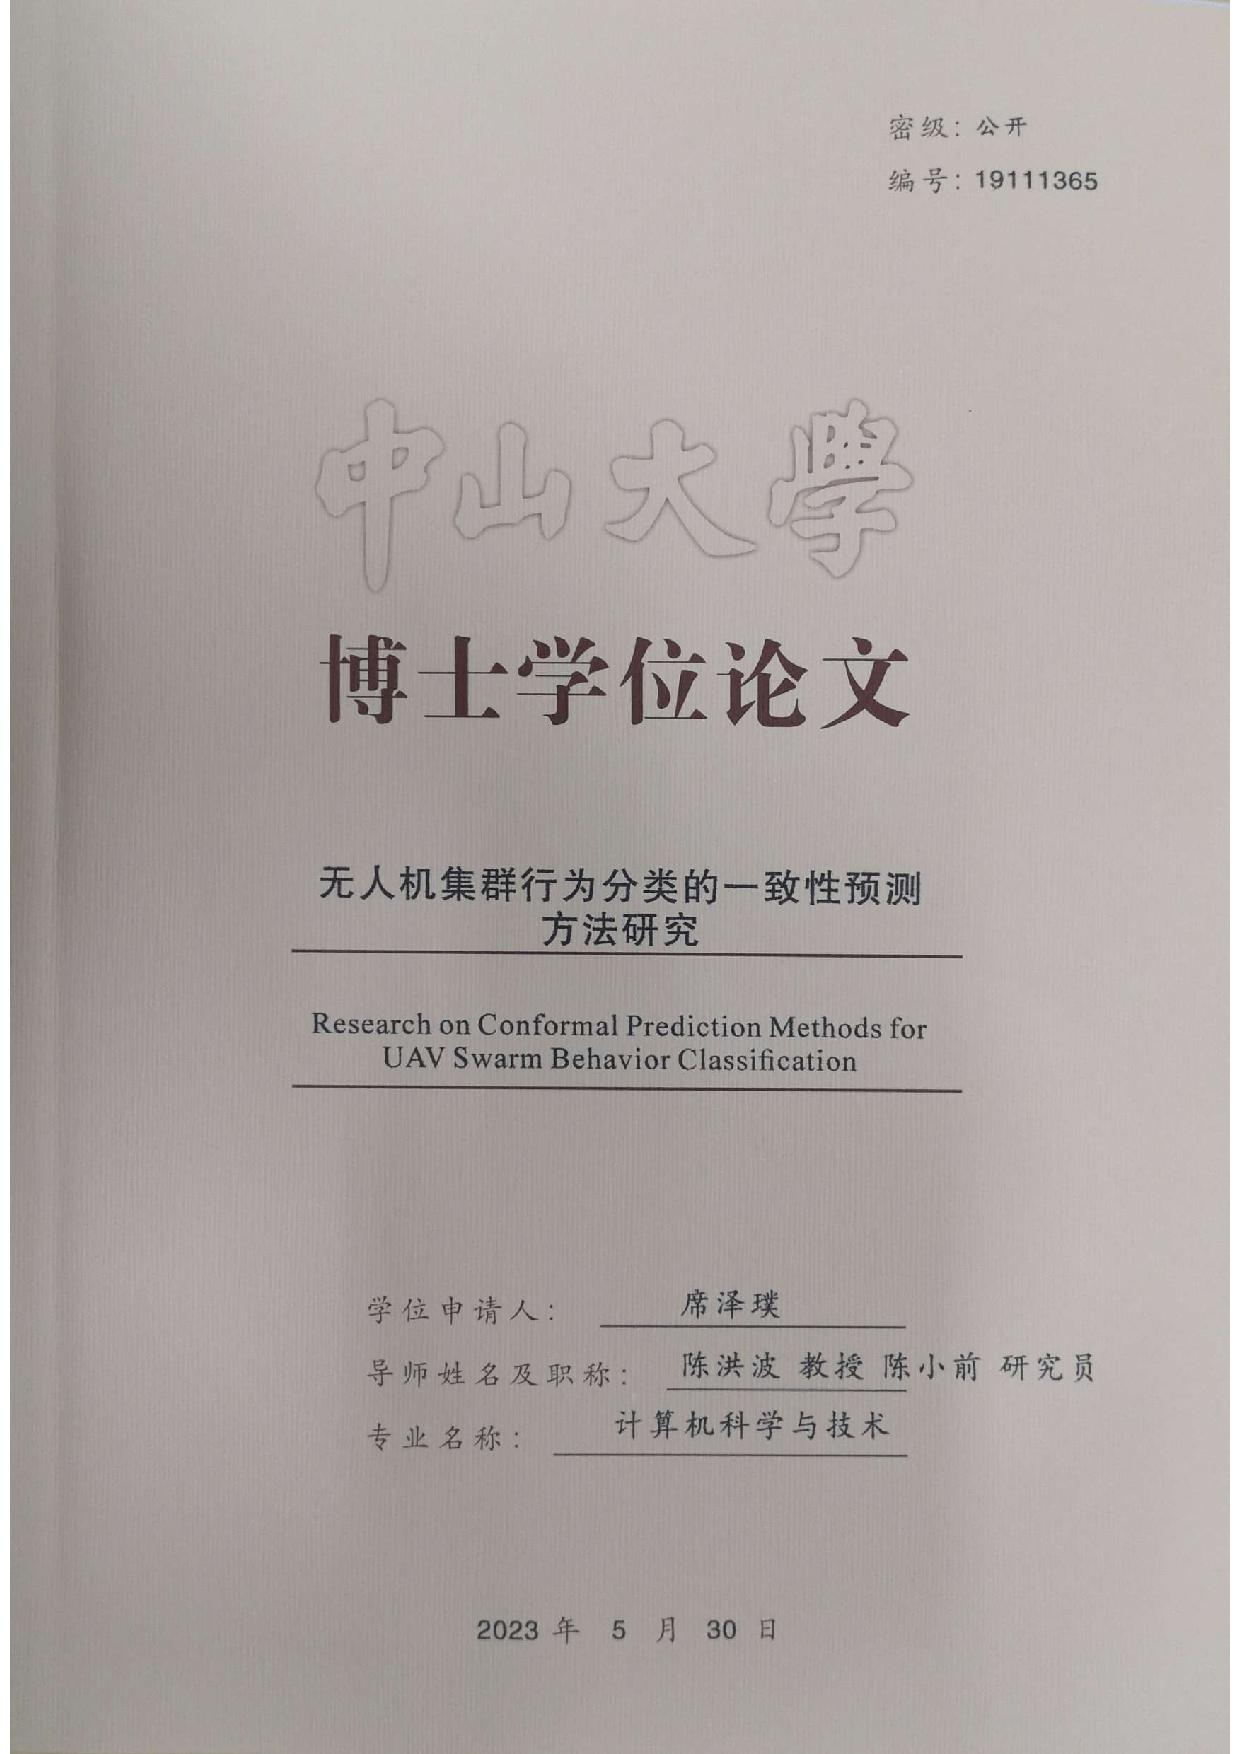
\includepdf[pages=-]{Tex/FM.pdf} % 更改封面为特定学校的封面
%-
%-> 中文摘要
%-
\intobmk\chapter*{摘\quad 要}% 显示在书签但不显示在目录
\setcounter{page}{1}% 开始页码
\pagenumbering{Roman}% 页码符号

具有高协同、复杂行为模式的无人机集群技术已经被广泛应用于各种军用和民用任务场景。面向不同目标的任务场景, 无人机集群系统需要按照不同的行为完成集群任务。针对无人机集群行为分类的研究为无人机集群意图推演提供具有重要建设性作用的前期信息支持。通过经验观测数据训练机器学习算法可以实现无人机集群行为分类并预测未知无人机集群行为。现有机器学习算法的输出只能提供单值预测, 忽视预测输出结果的置信程度。同时, 无人机集群行为数据随着时间变化会产生分布漂移问题, 现有机器学习算法忽视对分布漂移展开检测。再者, 目前大多数机器学习算法对训练数据样本需求量较大, 忽略在小样本下开展高精度预测模型的构建。

本文围绕利用机器学习实现无人机集群行为分类问题, 研究为分类算法的输出结果提供可信的不确定度量。针对数据分布随时间发生变化的难题, 本文研究无分布假设情形下开展数据分布漂移检测问题。在此基础上, 提出一种鞅保护分布算法提高机器学习模型的预测性能。面对小样本数据下要求实现无人机集群高精度分类难题, 本文研究使用特权信息范式为无人机集群行为分类提供高精度预测。

首先, 对于无人机集群行为分类研究中现有机器学习算法无法为其预测输出提供有效不确定量化难题, 本文提出采用一致性预测算法框架为利用机器学习算法实现无人机集群行为分类问题提供有效不确定量化。通过将机器学习算法的输出结果校正为有效p-值序列, 结合随机算法理论技术提出一种可建立在学习算法之上的无分布假设的有效不确定量化算法框架。本文提出的方法能够提供两种不确定量化模式, 一方面可以提供置信预测, 另一方面可以实现集合预测。通过无人机集群测试算例验证上述方法的有效性, 并对比分析所提方法的实用性。

其次, 从一致性预测理论出发, 针对无人机集群行为数据的分布随着时间发生变化的特点, 结合鞅理论提出无分布假设的分布漂移检测方法。本文提出的方法能够处理超高维数据的分布漂移检测并且无需任何分布假设。通过三种实际无人机集群行为数据, 验证所提鞅序列方法可以检测数据本身的分布随时间发生变化的问题。

此外, 本文将基于鞅序列的分布漂移检测理论应用于机器学习算法的顶层, 提出鞅保护分布算法。此算法在机器学习算法顶层构建保护带, 通过将随着时间变化的分布信息纳入考量来增强底层算法的学习泛化推广能力。研究结果表明, 本文提出的方法对于大多数机器学习算法都能够明显改善其预测能力。

最后, 针对常规机器学习算法大都需要建立在大样本学习机制上的问题, 结合实际工程应用中无人机集群行为数据稀缺的特点, 提出一种在小样本下实现高精度分类的算法。该算法能够将训练阶段可用但测试阶段不可用的信息(本文称之为特权信息)纳入模型, 使得在小样本下达到高精度预测的目标。研究结果表明, 本文提出的算法能够明显提升算法收敛速度, 使得无人机集群行为分类在小样本下也可以达到较高精度的预测效果。


\keywords{无人机集群系统, 集群行为分类, 一致性预测, 分布漂移检测, 使用特权信息学习}
%-
%-> 英文摘要
%-
\intobmk\chapter*{Abstract}% 显示在书签但不显示在目录

UAV swarm with high collaboration and complex behavior patterns has been widely applied in various military and civilian mission scenarios. UAV swarm system needs to complete different tasks according to different behaviors pattern in complex environment. We can make an effective statistical learning inference problem for recovering UAV swarm behavior pattern based on empirical data with the help of modern machine learning algorithms. However, most machine learning algorithms only output similarity measurement between each sample and there is no confidence measure for prediction of output value for particular new objects. At the same time, a common problem in UAV swarm applications of machine learning is that, soon after a prediction algorithm is trained, the distribution of the data may change, and the prediction algorithm may need to be retrained. Furthermore, most machine learning algorithms have a high demand for training data samples and have a low-precision prediction in small samples.

This thesis provide an effective distributions-free uncertainty quantification framework based on conformal prediction for hedging the prediction output. We also propose a distributions-free martingales framework to test distributions-shift. In particular, for speed up the convergence of learning, it is possible that we can build a new learning paradigm of pattern recognition algorithm based on learning using privileged information paradigm. 

Firstly, we propose Mondrian conformal prediction to provide exact valid error control for UAV swarm behavior classification. We adopt Mondrian conformal prediction methods to provide distributions-free uncertainty quantification. Our methods can be build on the top of any machine learning algorithms and provide exactly valid statistical inference. For the reliable machine learning of UAV swarm behavior pattern recognition with the help of Mondrian conformal prediction, we provide not only simple prediction with corresponding exact valid confidence and credibility measurements, but also exact valid set prediction under any user-specified significance level.

Secondly, we propose distributions-free methods to test distributions-shift under conformal test martingales for UAV swarm behavior datasets. The method proposed in this thesis have an effective distributions-shift detection for high-dimensional data without any distribution assumption. We test the proposed method on  three UAV swarm behavior datasets, it has been proven that the proposed martingale method provide an effective tools for distributions-shift detection.

Furthermore, based on the research of conformal test martingale, we find that it is important information that take into account the original order of UAV swarm behavior dataset. In this thesis, we introduce the martingale protected distribution methods that can be build on the top of any machine learning algorithm to integrated the original order of dataset to improve the performance of machine learning algorithm. 

Finally, we propose a new learning paradigm, called learning using privileged information (LUPI), to speed up the convergence of learning for UAV swarm behavior pattern recognition. It is remarkable that the privileged information that supply holistic description information is only available during the training stage rather than available during the test stage. When we introduce the privileged information for UAV swarm behavior pattern recognition, two experiments shows that the LUPI paradigm established well-performance predictive results.


\KEYWORDS{UAV Swarm Systems, Swarm Behaviors Classification, Conformal Prediction, Distributions-shift Detection, Learning Using Privileged Information}% 英文关键词
%---------------------------------------------------------------------------%
